\section{Context Awareness}
Improving the computers ability to access and understand a user's circumstances give developers more information for building  applications that respond and adapt to the user. A way to accomplish this is to not only use data given by the user but also use context information from the users environment. In earlier work Schilit and Thimer \cite{schilit1994disseminating} is defining context as locations, identities of close people and objects. This definition is too specific. It's not only locations that is interesting as context. According to Dey in \cite{dey2001understanding}, a better definition of context is:

\begin{quotation}
Context is a combination of any information that can be sensed or received by an entity which is useful to catch events and situations. \cite{dey2001understanding}
\end{quotation}

In other words context is information from an entity that gives specific information to increase the understanding of an events environment. An entity can be a person, place or a object that is relevant for the interaction. 

Humans implicitly use context information for making everyday decisions. An example of this is when a person is asking another person for directions to a place. The context in this conversation can be the location the persons are standing at and based on this the person giving the directions can either point or give a description of the sequence of right and left turns needed to reach the destination. By having this context information it is possible to give directions to the desired location. This kind of ability is therefore hard to transfer to human interaction with computers. One way of generating and sharing this context information on a large scale is through the use of smart telephones and other ubiquitous computing devices.

One such smartphone is the a Google Nexus 4 \cite{GoogleNexus} which contains, among other things, the sensors an accelerometer to detect acceleration, a GPS to receive location data, a gyroscope to detect rotation, a barometer to detect air pressure and a compass for direction and navigation. By applying sensor fusion \cite{Elmenreich02sensorfusion} other context data can be attained. An example of this would be combining a GPS with a barometer to faster detect altitude. Using these types of data, we can realize context-centric applications. Similar to the earlier example where a person was asking another person for directions to a place, the person can now ask for direction from his phone. The phone will collect context-information from the its GPS sensor and based on this location be able to give the directions. With this extra context information, we can create applications that are context aware. This idea of context awareness is summarized by Dey in \cite{dey2001understanding} as: 

\begin{quotation}
A system is context-aware if it uses context to provide relevant information and \slash or services to the user, where relevancy depends on the user's task. \cite{dey2001understanding}
\end{quotation}

An application is therefore context-aware if it is able to use context in order to adjust its behavior or the content it is providing. Example of context-awareness in applications is Google Latitude \cite{GoogleLatitude}. The application makes it possible for your friends to see your position on a map. Google Latitude uses the locations from a entity (mobile phone or computer) to update your position on the map. Another context-aware application from google is AdSense/AdWords. This application generates advertisement based on the context of the webpage the user have visited. Also Android is a good example of context-awareness in application. When a user rotates a smartphone or a tablet the operating system changes its orientation to landscape mode.

\begin{figure}[t] % To force on specific place use H
	\centering
    	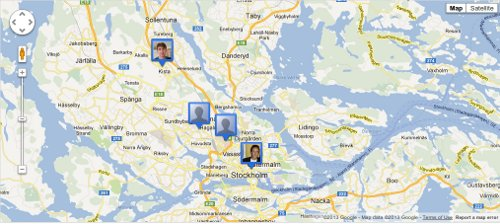
\includegraphics[scale=0.75]{part_2/context_awareness/latitude_pic.jpg}
		\caption{A picture of Google Latitude showing contacts shared positions.} 
\end{figure}

Context awareness can change classical scenarios into intelligent responsive scenarios by using context informations to behave in a special way. Common applications such as home automation can use information to turn on the light at home. In earlier implementations where applications did not use context information and users turn on lamps by manually pressing a button. In comparison, if the developer instead uses the context information the application can interact on information from sensors around the user. For example when a user enters his home the light will be turned on when the application detects his location from the users ubiquitous device. The developer can also use information that provides how the weather is outside, if it's sunny outside the application will act to this and it will not turn on the lights when the user enters his home, but if it's cloudy outside the application will turn on the light. Context awareness on a massive scale is gradually enabled by the advances in pervasive and ubiquitous computing.	

\begin{figure}[t] % To force on specific place use H
	\centering
    	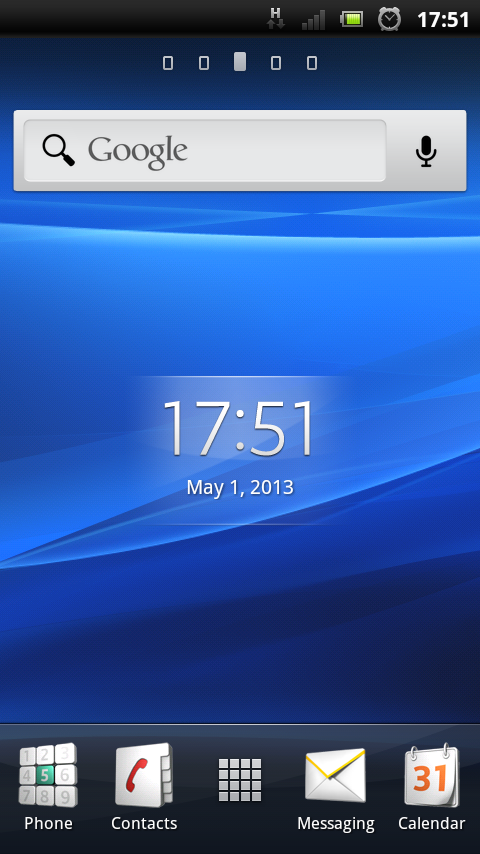
\includegraphics[scale=0.20]{part_2/context_awareness/screenshot_2013-05-01_1751.png}
    	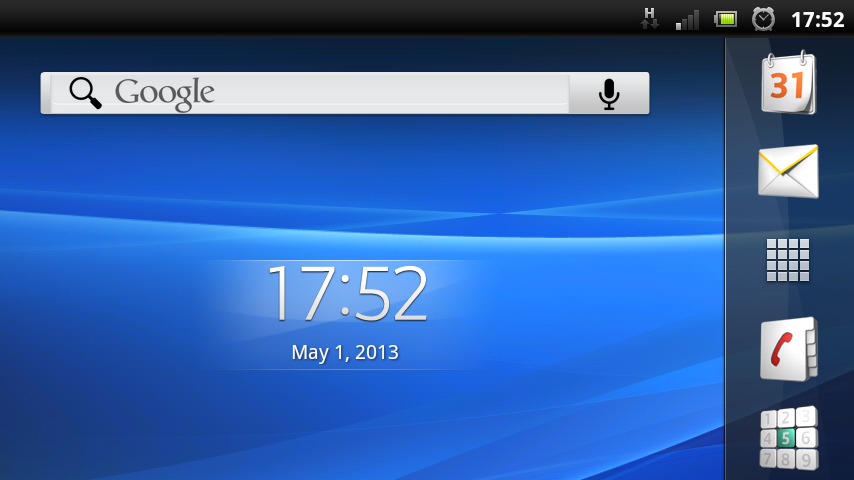
\includegraphics[scale=0.20]{part_2/context_awareness/screenshot_2013-05-01_1752.png}
		\caption{Android homescreen on a Sony Ericsson Xperia PLAY rotates based on context information from its sensors when the phone is 	physically rotated.} 
\end{figure}